%!TEX root = ../../Master.tex
\subsection{Location Fingerprinting}
In location fingerprinting, there are two main techniques that have been chosen for this project, "QR-code" and "RFID". Location fingerprinting is method of recognizing devices by giving them a electronic fingerprint, such as a unique id.

\subsubsection{QR-code} % (fold)
QR-codes are types of barcodes used for encoding text. The code is represented by black boxes on a white square grid background. All by how the boxes are arranged, the code will represent different data. See \cref{fig:qr}.

\begin{figure}
	\begin{center}
		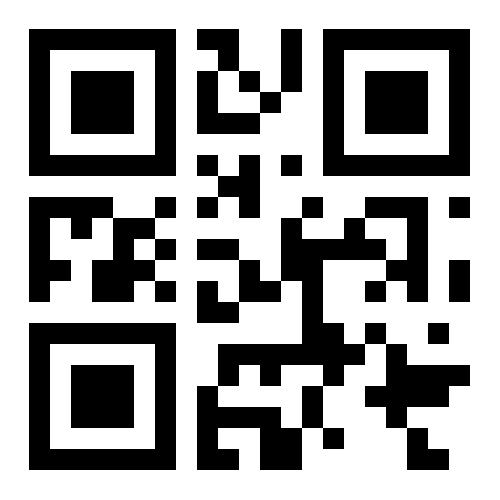
\includegraphics[width=0.5\textwidth]{qr_code}
	\end{center}
	\caption{An example of a QR code}
	\label{fig:qr}
\end{figure}

In order to read the data, a scanner has to be used. A camera from a smartphone can be used for this purpose, as long there are an app that supports this particular format. Such apps can be installed on nearly all smartphones\cite{QR_smart}. The QR-code can be used to directs users to websites, and are used often in different kind of commercial ways\cite{QR_url}.

It is easy to read the QR-code if you already have an app installed on your smartphone. It is also easy to make your own codes as Google have released a free tool to generate them\cite{QR_Google}. It is also rather easy to set up a QR-code system for a building, in a effective manor\cite{QR_easy}.

The relevance for this project is how it will take little to no time to set up\cite{QR_rel1}, and how some people already knows how use them as they are widely spread\cite{QR_spread}. Even if a code is damaged it will still be usable, all up to 30\% of the code can be missing\cite{QR_dama}. This also means it will be possible to implant images in the code and still have it working\cite{QR_image}.

A reason for not to use the codes could be that some users might exploit the system. If they print their own codes with links to certain websites it could be a very unpleasant experience for the other users\cite{QR_urlbad}. In worst case scenarios they could be used to steal personal information\cite{QR_information}.
In order for the codes to be efficient, they also have to placed at many locations at the hospital. The users should always be able to find them when they want to use them. This could leave to frustration if they seems to be nowhere to find for the user.


\subsubsection{RFID}
%Hvad er det?
%Output/Input?
%Hvorfor bruges det?
%Hvorofr er det relevant
%Hvorfor er det ikke relevant?

RFID (Radio Frequency Identification) is a radio technology that makes it possible, just like barcodes, to identify different objects. The main difference between these two technologies is that the barcode is a line of sight technology, and RFID is wireless, as long as it is within visible range of the a receiver. The readable distance varies depending on the type of RFID tag. The information exchanged can be in many different formats such as text, numbers, audio or video. The signal is send with via magnetic fields\cite{RFID_magnetic}.

There are different types of RFID tags each with different purposes. There are the active, semi passive and passive. The active tag can broadcast its radio waves to a RFID reader. The semi passive is different as it has no means of broadcasting on its own and will need the RFID reader to draw power from\cite{RFID_semiActive}. The passive tag does not have its own battery and will therefore need the RFID reader to supply power just like the semi-active tag. The semi-passive tag does however have a battery to supply its circuit with power\cite{RFID_AllTypes}.

The RFID tag is useful because it can help with identifying objects or persons who have a tag implanted\cite{RFID_FAQ}. A RFID reader can automatically find and read the tag if it is located inside the tags range. Wallmart uses RFID to automatically store data when curtain goods arrive, which will save them time and energy\cite{RFiD_inc}. Passive RFID tags have also been developed to be used on cars in order to identify them. It is being considered for cross border control other uses as roll toll collection\cite{RFID_car}. This will make it easier for the driver if he/she can automatically pay tolls. This is used in the Danish Brobizz\cite{RFID_brobizz}   

In this project the tags could be used to position the users as they go trough the building. The active tags could be on the user or device, and when they comes near a reader the reader could tell a server where the tag have been read. In that way the user will be repositioned every time they comes near a "checkpoint". These "checkpoint" could be placed every time there was a turn or a door, as the route then could be planned from that position.

A problem with this and the QR-code solution would be that the users will not be positioned when they are in a middle of a hallway without doors, as no readers will be near them. To get around this problem, the complex should be filled with readers everywhere. This could evolve into a major project if all the hallways have been plastered.

\subsubsection{Wi-Fi} \label{wifitech}
Wi-Fi is a technology that uses radio waves to transfer data between electronic devices. Computers and handheld devices make use of Wi-Fi, together with many other electronic devices \cite{wifi_devices}.

Wi-Fi can be used in location fingerprinting using triangulation. This works because every Wi-Fi hotspot has an unique id and a known location. An estimated position of a Wi-Fi receiver can be calculated based on the signal strength to every Wi-Fi hotspot. It is then possible to calculate a position  \cite{Liu2007}.

Wi-Fi can connect to the internet via a wireless access point such as a router. Wi-Fi allows places that normally would not have internet connection, like sheds or gardens, to connect. This is possible as the router or wireless access point will allow the device to get a connection.

This is widely used as they serve as an convenient way of getting internet access. They are fairly easy to set up and used widely in the private homes and also used at a greater scale such as an airport \cite{wifi_works}. It is an convenient way of getting internet access as the user is in no need of getting a cable that physically have to be connected to a router.

It is relevant for this project as there have been invested in installing Wi-Fi hotspots at the Danish hospitals \cite{wifi_hospi}. This means it would be possible to set up a service that will connect trough these hotspots.

A problem with Wi-Fi is how, as by Danish law, the hospital will have to log data from the users who connect to it \cite{wifi_log}. In order to only log the users who are using the Wi-Fi, a password would be optimal as it will prevent people bypassing the complex from automatically connecting. The range is also a limitation as typical routers will support a range of 46 meters indoor \cite{wifi_range}. Walls will reduce the strength of the signal, which means some areas of the complex might no have a good enough connection \cite{wifi_wall}. Handheld devices consumes more power when Wi-Fi is active, and quickly drains the battery as data is send and received \cite{wifi_batt}. The amount of power used is reduces as the device goes into a low power mode, which is activated once it has no more data to send. It goes into hight power mode when it is sending/receiving data and stays there for the duration of which it is sending/receiving the data.

